\section{Reward}\label{sectionReward}
The reward is important in reinforcement learning because the agent must maximize the reward for learning how to act in the environment. Consider teaching a dog a new trick: you cannot tell it what to do, but you can reward/punish it if it does the right/wrong thing. The dog should figure out what it did to get the reward/punishment, which is known as the credit assignment problem \cite{reward_small}. We can use a similar method to train the agent how to drive a car. More about the reward can be read in \Cref{TheorBkgdRL}.  

In this project, two reward function is compared, for learning the agent how to drive a car in the TORCS environment - see more of the environment in \Cref{sec:TORCS}.  

\subsection*{First reward function}
The first reward function used in this project is the reward function from the paper \cite{DBLP:journals/corr/LillicrapHPHETS15}: \\
\textit{"For the Torcs environment we used a reward function which provides a positive reward each step for the velocity of the car projected along the direction and a penalty of -1 for collisions. Episodes were terminated if progress was not made along the track after 500 frames."}\\
To understand this a figure to illustrate the reward can be seen on \Cref{fig:Reward_paper}.

\begin{figure}[H]
	\centering
	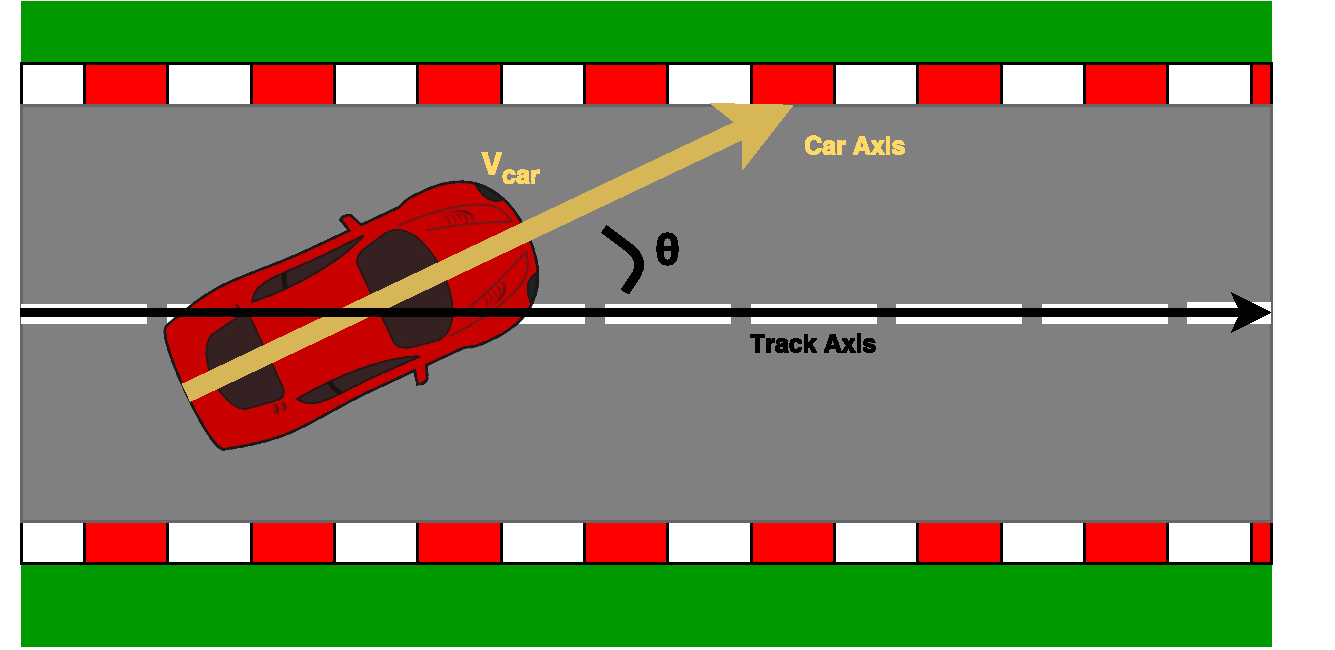
\includegraphics[width=1\textwidth]{Figures/Result/Reward_paper.pdf}
	\caption{Explanation of the reward used in the paper \cite{DBLP:journals/corr/LillicrapHPHETS15} }
	\label{fig:Reward_paper}
\end{figure}

The reward function here is:
\begin{equation}
Reward = V_{car} \cdot cos(\theta) 
\end{equation}
The idea this reward function uses is getting a reward for how fast the car drives ($V_{car}$), in the center of the road. The agent gets more reward when the car is driving fast at the center of the road, and less reward when the car is driving fast away from the center of the road. 

\subsection*{Second reward function}
After testing the first reward function, it was concluded, that this reward function didn't perform as expected. Because the reward function is important for learning, another reward function is tried. This reward function is taken from the blog \cite{DDPG_Torcs}. Here it uses the same idea, that the reward should be bigger if the car drives fast in the center of the road, and less reward when it is away from the center. The reward function looks like this:

\begin{equation}
\label{eq:reward_2}
Reward = V_{car} \cdot cos(\theta) - V_{car} \cdot sin(\theta) - V_{car} \cdot \mid trackPos\mid 
\end{equation}
The TrackPos gives percent the car is away from the center of the road. Which is useful in this reward function, because it is wanted that the car should be near the center of the road.  

In \Cref{eq:reward_2} the first term ($V_{car} \cdot cos(\theta)$) want to maximum longitudinal velocity, second term ($V_{car} \cdot sin(\theta)$) try to minimize transverse velocity. It penalize the AI if it constantly drives away from the center of the road in the third term ($V_{car} \cdot \mid trackPos\mid$).

Here it sees the agent learns how to drive, and this is the reward function where the best results came from. It has to improve the stability of the training. 

To test the two reward functions influence on the learning, all other parameters stays as described in the introduction to this \Cref{cha:Result}. Thereby it should be possible to only see the influence of the two different reward functions. 

To compare both reward functions a graph is created, this graph can be seen on \Cref{fig:change_of_Reward_reward_graph}:

\begin{figure}[H]
	\centering
	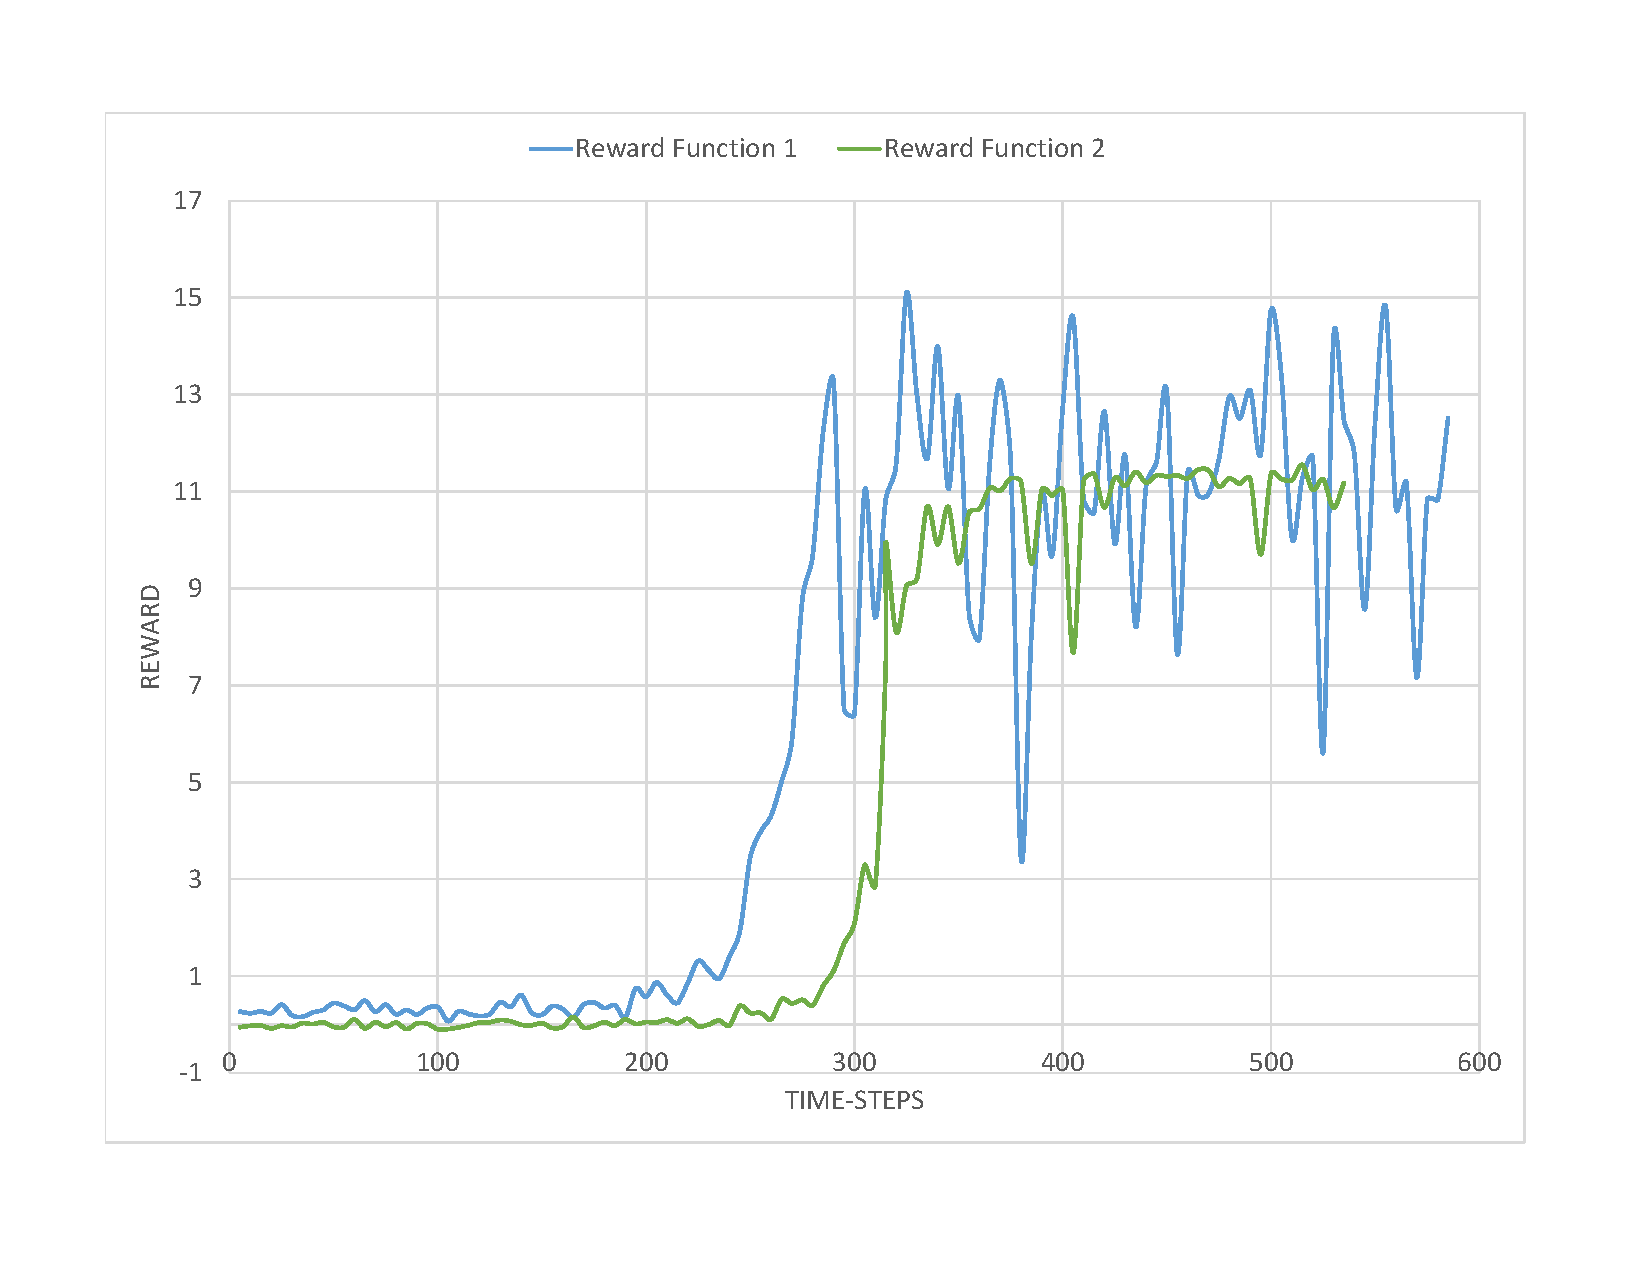
\includegraphics[width=1\textwidth]{Figures/Result/change_of_Reward_reward_graph.pdf}
	\caption{Comparison of the two different reward functions with the reward getting from the environment}
	\label{fig:change_of_Reward_reward_graph}
\end{figure}

The \Cref{fig:change_of_Reward_reward_graph} shows the average total reward of 5 time-steps (episodes). The reward after every step (state) is added together to get the total reward. The total reward is the reward when an episode is finished. An episode is finished, when the car is not on the road, the car is driving backward or the car has finished a lap.   

On the graph in \Cref{fig:change_of_Reward_reward_graph} shows that both reward function have the wanted effect, and the first reward function converge faster than the second reward function around 250 time-steps and the second reward function converge around 320 time-steps. The negative side of the first reward function is it looks more unstable than the second reward function. This is seen by looking at the graphs converge value, which is not as constant on the first reward function, as on the second reward function. 

The stability issue of the learning can also be seen on the driving car in the TORCS environment. Here it looks like the first reward function drives close to the edge of the road, and learns how to follow the red and white striped edges. In the second reward function, the car learns to drive near the center of the road, where the car is more following the white lines in the center of the road. 

The second reward function works best, it is the reward function which has been used in the final algorithm for the agent.
 
